\documentclass{article}

\usepackage{graphicx}
\usepackage{tikz}
\usepackage{tikzsymbols}
\usetikzlibrary{calc,patterns,shapes.geometric}
\pagestyle{empty}
\usepackage[margin=0pt]{geometry}
\geometry{papersize={14in,12in}}

\def\centerarc[#1](#2)(#3:#4:#5){\draw[#1] ($(#2)+({#5*cos(#3)},{#5*sin(#3)})$) arc (#3:#4:#5);}

\begin{document}
	\begin{figure}
		\centering
		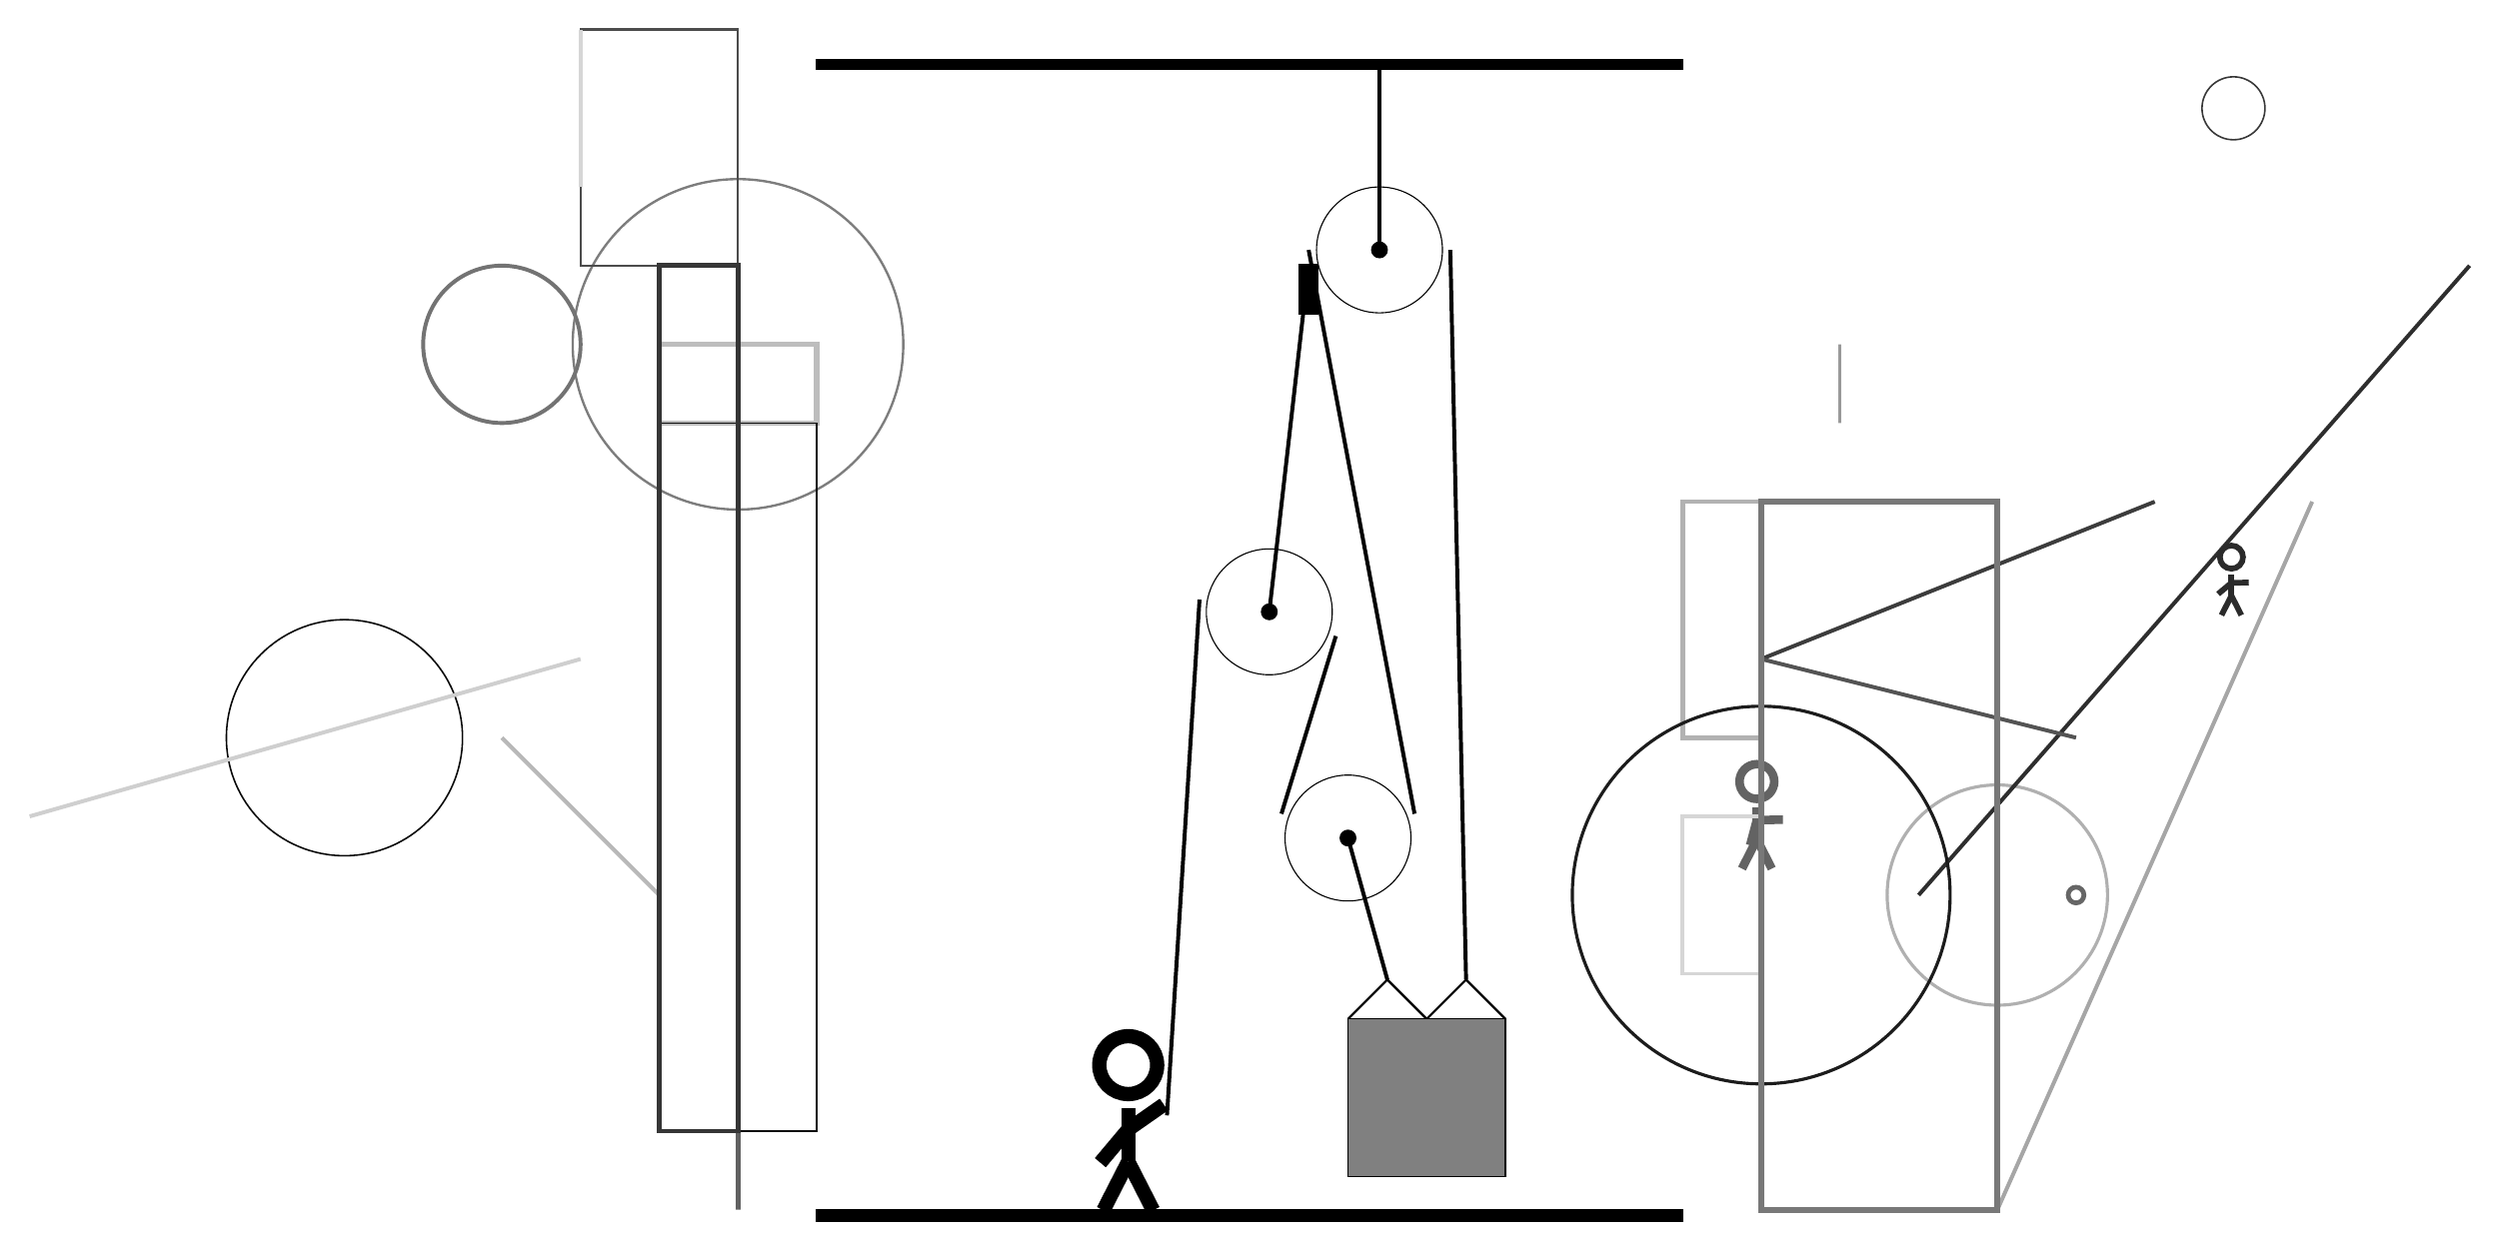
\begin{tikzpicture}
			%%%%% START %%%%%
			
			\draw[fill=black] (-6, 11.5) rectangle (5, 11.625);
			
			\draw (-0.25, 4.6) circle (0.8);
			\draw[fill=black] (-0.25, 4.6) circle (0.1);
			
			\draw [line width=0.4mm, color=black!31](9, 1) circle (1.4);
			
			\draw [line width=0.2mm, color=black!78](12, 11) circle (0.4);
			\node[line width=0.4mm, color=black!61] at (6, 2) {\Strichmaxerl[6][75][1]};
			\draw[line width=0.5mm, color=black!28](-8, 1) -- (-10, 3);
			\draw [line width=0.3mm, color=black!51](-7, 8) circle (2.1);
			
			\draw[line width=0.5mm, color=black!82](8, 1) -- (15, 9);
			\draw[line width=0.4mm, color=black!40] (7, 7) rectangle (7, 8);
			\draw[line width=0.7mm, color=black!26] (-6, 8) rectangle (-8, 7);
			\draw[line width=0.3mm, color=black!70] (-7, 9) rectangle (-9, 12);
			\draw[line width=0.3mm, color=black!66] (6, 1) rectangle (6, -1);
			\draw[line width=0.5mm, color=black!35](9, -3) -- (13, 6);
			\draw [line width=0.2mm, color=black!97](-12, 3) circle (1.5);
			\draw[line width=0.6mm, color=black!30] (6, 3) rectangle (5, 6);
			
			\draw [line width=0.5mm, color=black!55](-10, 8) circle (1.0);
			\node[line width=0.3mm, color=black!83] at (12, 5) {\Strichmaxerl[4][40][1]};
			\draw[line width=0.2mm, color=black!95] (-6, 7) rectangle (-8, -2);
			
			\draw[line width=0.6mm, color=black!62] (-7, 2) rectangle (-7, -3);
			\draw[line width=0.5mm, color=black!19](-9, 4) -- (-16, 2);
			\draw[line width=0.5mm, color=black!16] (6, 0) rectangle (5, 2);
			\draw[line width=0.5mm, color=black!76](6, 4) -- (11, 6);
			\draw[line width=0.6mm, color=black!79] (-7, -2) rectangle (-8, 9);
			
			\draw [line width=0.4mm, color=black!89](6, 1) circle (2.4);
			\draw[line width=0.5mm, color=black!16](-9, 10) -- (-9, 12);
			\draw[line width=0.5mm, color=black!67](6, 4) -- (10, 3);
			\draw [line width=0.6mm, color=black!60](10, 1) circle (0.1);
			
			\draw[line width=0.7mm, color=black!53] (6, 6) rectangle (9, -3);
			
			
			\draw (0.75, 1.725) circle (0.8);
			\draw[fill=black] (0.75, 1.725) circle (0.1);
			
			\draw (1.15, 9.2) circle (0.8);
			\draw[fill=black] (1.15, 9.2) circle (0.1);
			\draw[very thick] (1.15, 9.2) -- (1.15, 11.5);
			
			\draw[thick]  (0.75, -0.575) -- (1.25, -0.075) -- (1.75, -0.575) -- (2.25, -0.075) -- (2.75, -0.575);
			\draw[fill=black!50] (0.75, -0.575) rectangle (2.75, -2.575);
			
			\draw[line width=0.5mm] (-0.25, 4.6) -- (0.25, 9.0);
			\draw[line width=0.5mm, fill=black](0.15, 8.4) rectangle (0.35, 9.0);
			\draw[line width=0.5mm] (-1.55, -1.8) -- (-1.1363, 4.7562);
			\centerarc[line width=0.5mm](-0.25, 4.6)(-20:170:0.9);
			\draw[line width=0.5mm] (0.5957, 4.2922) -- (-0.0957, 2.0328);
			\centerarc[line width=0.5mm](0.75, 1.725)(160:380:0.9);
			\draw[line width=0.5mm] (1.5957, 2.0328) -- (0.25, 9.2);
			\draw[line width=0.5mm](0.75, 1.725) -- (1.25, -0.075);
			\centerarc[line width=0.5mm](1.15, 9.2)(0:180:0.9);
			\draw[line width=0.5mm] (2.05, 9.2) -- (2.25, -0.075);
			
			\node at (-2, -1.9) {\Strichmaxerl[10][50][35]};
			
			\draw[fill=black] (-6, -3) rectangle (5, -3.15);
			
			%%%%% END %%%%%
		\end{tikzpicture}
	\end{figure}	
\end{document}